\documentclass[]{article}

% include Packages
%\usepackage{pdfpages}
\usepackage{amsmath,amssymb}
\usepackage{amsthm}
\usepackage{xcolor}
\usepackage{graphicx}
\usepackage{float}

% Formatting text ranges
\setlength{\textwidth}{450pt}
\setlength{\textheight}{685pt}
\setlength{\topmargin}{-40pt}
\setlength{\hoffset}{-15mm}

% Define Theorem environments
\newtheorem{theorem}{Theorem}
\newtheorem*{theorem*}{Theorem} % allow not enumerated theorems
\newtheorem{definition}{Definition}
\newtheorem{remark}{Remark}
\newtheorem{lemma}{Lemma}
\newtheorem{corollary}{Corollary}

% Define custom commands
\newcommand{\yopt}{y^*}
\newcommand{\todo}{{\color{red} TODO!}}
\newcommand{\ind}[2]{{#1}_{\mathrm{#2}}}
\newcommand{\trp}{^T}
\newcommand{\fx}{f(x)}
\newcommand{\fsigx}{f(\sigma x)}
\newcommand{\fxtrp}{f \trp (x)}
\newcommand{\xone}{x_1}
\newcommand{\xtwo}{x_2}
\newcommand{\xj}{x_j}
\newcommand{\xjplus}{x_{j+1}}
\newcommand{\xk}{x_k}
\newcommand{\uj}{u_j}
\newcommand{\uk}{u_k}
\newcommand{\ui}{u_i}
\newcommand{\dotx}{\dot x}
\newcommand{\dotxone}{\dotx_1}
\newcommand{\dotxtwo}{\dotx_2}
\newcommand{\Rn}{\mathbb{R}^n}
\newcommand{\Nset}{\mathbb{N}}
\newcommand{\forntoinf}{\overset{n \rightarrow \infty}{\longrightarrow}}
\newcommand{\jacf}{\dfrac{\partial }{\partial x} \fx}
\renewcommand{\brack}[1]{\left[ #1 \right]}
\newcommand{\parenth}[1]{\left( #1 \right)}
\newcommand{\jacfbrack}{\brack{\jacf}}
\newcommand{\matleq}{\preccurlyeq}
\newcommand{\norm}[1]{\parallel \! \! #1 \! \! \parallel}
\newcommand{\partialx}{\frac{\partial}{\partial x}}
\newcommand{\dsig}{\mathrm{d} \sigma}
\newcommand{\intsigma}{\int_{0}^{1} \partialx \fsigx x \dsig}
\newcommand{\Qx}{Q(x)}
\newcommand{\Vx}{V(x)}
\newcommand{\xtrp}{x \trp}
\newcommand{\gammaxsig}{\gamma(x,\sigma)}
\newcommand{\xn}{x_n}
\newcommand{\xnull}{x_0}
\newcommand{\unull}{u_0}
\newcommand{\xN}{x_N}
%\newcommand{\xk}{x_k}
\newcommand{\xeq}{x^{\mathrm{e}}}
\newcommand{\xeqone}{x^{\mathrm{e}}_1}
\newcommand{\xeqtwo}{x^{\mathrm{e}}_2}
%\newcommand{\uk}{u_k}
\newcommand{\xtrpn}{x_n \trp}
\newcommand{\fxn}{f(\xn)}
\newcommand{\dotVx}{\dot{V}(x)}
\newcommand{\dVdtx}{\frac{\mathrm{d} V(x)}{\mathrm{d} t}}
\newcommand{\partialVx}{\frac{\partial V(x)} {\partial x}}
\newcommand{\matricks}[4]{\begin{pmatrix}#1 & #2 \\ #3 & #4 \end{pmatrix}}
\newcommand{\twovector}[2]{\begin{pmatrix}{ #1 }\\{ #2 }\end{pmatrix}}
\newcommand{\Ad}{A_d}
\newcommand{\Bd}{B_d}
\newcommand{\xkplus}{x_{k+1}}
%\newcommand{\dotx}{\dot{x}}
\newcommand{\tk}{t_{k}}
\newcommand{\tkplus}{t_{k+1}}
\newcommand{\Aeul}{\ind{A}{eul}}
\newcommand{\Beul}{\ind{B}{eul}}
\newcommand{\optmin}{\mathrm{min}.}
\newcommand{\Aeq}{\ind{A}{eq}}
%\newcommand{\Aeqx}{\ind{A^x}{eq}}
%\newcommand{\Aequ}{\ind{A^u}{eq}}
\newcommand{\beq}{\ind{b}{eq}}
\newcommand{\Aeqx}{\Aeq^x}
\newcommand{\Aequ}{\Aeq^u}
\newcommand{\Aineq}{\ind{A}{{  in}}}
\newcommand{\bineq}{\ind{b}{{  in}}}
\newcommand{\xbar}{\bar{x}}
\newcommand{\xtilde}{\tilde{x}}
\newcommand{\vectorthree}[3]{\begin{pmatrix}
		#1 \\ #2 \\ #3
\end{pmatrix}}
\newcommand{\vectortwo}[2]{\begin{pmatrix}
		#1 \\ #2
\end{pmatrix}}
\newcommand{\half}{\frac{1}{2}}
\newcommand{\grad}{\nabla}
\newcommand{\N}{\mathbb{N}}
\newcommand{\R}{\mathbb{R}}
%\newcommand{\Rn}{\mathbb{R}^n}
\newcommand{\Rm}{\mathbb{R}^m}
\newcommand{\Rp}{\mathbb{R}^p}
\newcommand{\Fx}{F(x)}
\newcommand{\jac}{J}
\newcommand{\jacF}{\jac F}
\newcommand{\inv}{^{-1}}
\newcommand{\fnull}{f_0}
\newcommand{\X}{\mathcal{X}}
\newcommand{\U}{\mathcal{U}}
\newcommand{\writeset}[1]{\{#1\}}
\newcommand{\Vk}{V_k}
\newcommand{\Vopt}{\Vind{*}}
\newcommand{\Vind}[1]{V^#1}
\newcommand{\Vone}{\Vind{1}}
\newcommand{\Vtwo}{\Vind{2}}
\newcommand{\Vzero}{\Vind{0}}
\newcommand{\Vnull}{\Vind{0}}
\newcommand{\Vkplus}{V_{k+1}}
\newcommand{\Vtil}{\tilde{V}}
\newcommand{\minVit}[6]{\min_{u \in \U} \writeset{#1+0.9\Vk(\xi_{#2}), #3+0.9\Vk(\xi_{#4}),#5+0.9\Vk(\xi_#6) }}
\newcommand{\VstateVal}[2]{V(\xi_#1) &= #2}
\newcommand{\kstateVal}[2]{k(\xi_#1) &= #2}
\newcommand{\util}{\tilde{u}}
\newcommand{\uopt}{u^*}
\newcommand{\lambdamin}{\lambda_{\mathrm{min}}}
\newcommand{\lambdamax}{\lambda_{\mathrm{max}}}
\newcommand{\Xf}{\X_f}
%opening
\title{Optimal Control WS20/21: Homework 2}
\author{Daniel Bergmann}

\begin{document}

\maketitle

\subsection*{Problem 1}
		\begin{enumerate}
			\item[a)] Formulating the problem as an discrete-time, infinite-horizon o. c. problem yields
				\begin{equation}
				\begin{aligned}
				& \underset{u_0,u_1,\dots}{\text{min.}}
				& & \sum_{k=0}^{\infty}\alpha^k \fnull(\xk,\uk) = \sum_{k=0}^{\infty}  0.9^k \fnull(\xk,\uk)\\
				& \text{subject to}
				& & \xkplus = f(\xk,\uk),\\
				& & & \xk \in \X = \writeset{\xi_1,\dots,\xi_8},\\
				& & & \uk \in \U = \writeset{0,1,2},\\
				& & &\xnull = \xi_1,\\ 
				\end{aligned}
				\end{equation}
				where the dynamics $ f: \X \times \U \longrightarrow \X $ are defined by the arrows in the graph.
				
				The Value function iteration is defined by the Bellman operator
				\begin{equation} \label{eq:BellmanOp}
					\Vkplus(x) = T\Vk(x) = \underset{u \in \U}{\min} \writeset{\fnull(x,u) + \alpha \Vk(x)}  \quad \text{with} \quad \alpha= 0.9.
				\end{equation}
				Evaluated for this particular problem, this yields
				\begin{align}
					\begin{split}
						\Vkplus(\xi_1) &= \min_{u \in \U} \writeset{1+0.9 \Vk(\xi_2),1+0.9\Vk(\xi_3)},\\
						\Vkplus(\xi_2) &= \min_{u \in \U} \writeset{3+0.9 \Vk(\xi_7),6+0.9\Vk(\xi_5),3+0.9\Vk(\xi_4)},\\
						\Vkplus(\xi_3) &= \min_{u \in \U} \writeset{1+0.9\Vk(\xi_4), 2+0.9\Vk(\xi_6),3+0.9\Vk(\xi_5) },\\
						\Vkplus(\xi_4) &= \minVit{2}{7}{6}{8}{3}{6},\\
						\Vkplus(\xi_5) &= \minVit{0}{4}{0}{4}{1}{6},\\
						\Vkplus(\xi_6) &= \minVit{5}{1}{1}{7}{1}{8},\\
						\Vkplus(\xi_7) &= \minVit{2}{8}{2}{8}{2}{8},\\
						\Vkplus(\xi_8) &= \minVit{0}{8}{0}{8}{0}{8},
					\end{split}
				\end{align}
				starting with an arbitrary inital value function $ \Vnull: \X \longrightarrow \R $.
			\item[b)]
				Value function $ V:\R^8 \longrightarrow \R $, obtained after 1000 value function iterations:\\
				
				\begin{align}
					\begin{split} \label{eq:VVals}
				    \VstateVal{1}{3.61}\\
					\VstateVal{2}{4.80}\\
					\VstateVal{3}{2.90}\\
					\VstateVal{4}{3.80}\\
					\VstateVal{5}{1.90}\\
					\VstateVal{6}{1.00}\\
					\VstateVal{7}{2.00}\\
					\VstateVal{8}{0.00}.
					\end{split}
				\end{align}
				The values in \eqref{eq:VVals} induce the following state feedback:\\
				\begin{align} \label{eq:kVals}
					\begin{split}
					\kstateVal{1}{u_2}\\
					\kstateVal{2}{u_1}\\
					\kstateVal{3}{u_1}\\
					\kstateVal{4}{u_1}\\
					\kstateVal{5}{u_2}\\
					\kstateVal{6}{u_2}\\
					\kstateVal{7}{u_0}\\
					\kstateVal{8}{u_0}.
					\end{split}
				\end{align}
			For the initial state $ \xnull = \xi_1 $, the state-feedback given in \eqref{eq:kVals} yields the optimal input sequence
			\[ u^* = \left(2 \quad 1 \quad 2\right), \] that steers the state to the terminal state $ \xi_8  $ via the route $ \xi_1,\xi_3,\xi_6,\xi_8 $.
			
			
			\item[c)] We suppose
			\begin{equation}
				\Vnull(\xi) \leq T\Vnull(\xi) \quad \forall_{\xi \in \X} \label{eq:InitAssumption},
			\end{equation}
			for an initial function $ \Vnull $ for a value function iteration with the Bellman Operator, defined in \eqref{eq:BellmanOp}.
			From the lectures, we have the following properties.
			\begin{align}
				\norm{T\Vone - T\Vtwo}_\infty &\leq \alpha \norm{\Vone - \Vtwo}_\infty \quad &\text{(Contraction)} \label{eq:contraction}\\
				\Vone(\xi) &\leq \Vtwo(\xi) \quad \forall_{\xi \in \X} \Longrightarrow T\Vone(\xi) \leq T\Vtwo(\xi) \quad \forall_{\xi \in \X} \quad &\text{(Monotonicity)} \label{eq:monotonicity}\\
				\Vopt \text{ solves the Bellman Equation }&  \Vopt \text{ is the Value function, since we have discounted costs.} \label{eq:sufficientBE}
			\end{align}
			First we show, that the iteration converges to the value function of the problem. Since \eqref{eq:contraction} holds and   $ \alpha \in (0,1) $,we deduce the convergence of  $ \writeset{\Vk}_{k \in \N} $ by the Banach-Fixed-Point-Theorem. Since we have such a limit $ \lim\limits_{k \rightarrow \infty} \Vk \longrightarrow \Vopt $, it has to satisfy the fixed point property $ T\Vopt = \Vopt $. Hence it satisfies the Bellman equation and \eqref{eq:sufficientBE} verifies $ \Vopt $ as the value function of our problem.
			
			Second, it remains to show that $ \Vnull(\xi) \leq \Vopt(\xi) \forall_{\xi \in \X} $ holds.\\
			By assumption \eqref{eq:InitAssumption} and the monotonicity property \eqref{eq:monotonicity}, we infer inductively, that $ \Vk(\xi) \leq \Vkplus(\xi) $ for all $ \xi \in \X $. Thus, the sequence $ \writeset{\Vk(\xi)}_{k\in \N_0} $ is non-decreasing for any $ \xi \in \X $. This proves the claim $ \Vnull(\xi) \leq \Vopt(\xi) \forall_{\xi \in \X } $.
			
			\item[d)] Maximization Problem:
			
			\begin{equation} \label{eq:maxProblem}
			\begin{aligned}
			& \underset{V(\xi_1),\dots,V(\xi_n)}{\text{max.}}
			& & \sum_{k=0}^{n} V(\xi_i)\\
			& \text{subject to}
			& & V(\xi_i)  \leq TV(\xi_i)\quad\forall_{ i= 1,\dots,n}.\\
			\end{aligned}
			\end{equation}
			To show: $ \Vopt $ is a solution to the maximization problem given above.
			Proof by contradiction. Suppose, there exists an admissible Function $ \Vtil :\R^n \longrightarrow \R$ with \begin{equation}
				\Vtil(\xi_i) > \Vopt(\xi_i) \label{eq:counter}
			\end{equation}  for at least one $ i \in \writeset{1,\dots,n} $. Since $ \Vtil $ is admissible for the given max. problem, we know that $ \Vtil(\xi_i) \leq T\Vtil(\xi_i) \quad \forall_{i\in \writeset{1,\dots,n}} $. From excercise c) we know, that hence $ \Vtil(\xi_i) \leq T^k\Vtil(\xi_i) \leq \Vopt(\xi_i)$ holds for all $ i \in  \writeset{1,\dots,n} $ and for all $ k \in \N $.  This clearly contradicts \eqref{eq:counter}. Thus, $ \Vopt $ maximizes the objective of the given problem.
			
			\item[e)] Transform \eqref{eq:maxProblem} into
			\begin{equation} \label{eq:maxProblemArgmax}
				\begin{aligned}
				 \Vopt= &\underset{V(\xi_1),\dots,V(\xi_n)}{\text{ arg max.}}
				& & \sum_{k=0}^{n} V(\xi_i)\\
				& \text{subject to}
				& & V(\xi_i)  \leq \fnull (\xi_i,u)+ \alpha V(f(\xi,u))\\
				& & &\forall_{u\in \U(\xi_i)} \forall_{ i= 1,\dots,n}.\\
				\end{aligned}
			\end{equation}
			As shown in d), $ \Vopt $ maximizes the objective of problem \eqref{eq:maxProblem}. It remains to show, that the constraints of problems \eqref{eq:maxProblem} and \eqref{eq:maxProblemArgmax} are equivalent. The operator $ T $ is defined by the Bellman Equation, as written in \eqref{eq:BellmanOp}.
			We have
			\begin{align}
			\begin{split} \label{eq:ineqConstraint}
				V(\xi_i)  \leq TV(\xi_i) &= \underset{u \in \U}{\min} \writeset{\fnull(\xi_i,u) + \alpha \Vk(\xi_i)}\\
				&\leq \fnull(\xi_i,\util) + \alpha \Vk(\xi_i)
			\end{split}
			\end{align}
			for any input signal $ \util \in \U $. This arises directly from the definition of the minimum. Thus, \eqref{eq:maxProblem} and \eqref{eq:maxProblemArgmax} denote the same problem.
			
			It remains to formulate this as a linear program
			\begin{equation} \label{eq:maxProblemArgmax}
				\begin{aligned}
				\Vopt &=  \underset{V}{\text{ arg max.}}
				& & c\trp V\\
				& \text{subject to}
				& & AV \leq b.\\
				\end{aligned}
			\end{equation}
			
			 With $ V = (V(\xi_1),\dots,V\xi_n)\trp $, the objective $\mathrm{max.} \ \sum_{k=0}^{n} V(\xi_i) $ is the same as $ \mathrm{min.} \ c\trp V $ with \[ c = -(1,\dots,1)\trp \in \Rn. \]
			 Now we rewrite the constraints as a linear inequality $ AV = b $.
			 
			 For a state $ \xi_i \in \X $, the inequality
			 \begin{align}
%			 \begin{split}
			  	&V(\xi_i) \leq \fnull (\xi,u) +  \alpha V(f(\xi_i,u))\notag\\
			 \Longleftrightarrow \ &V(\xi_i) - \alpha V(f(\xi_i,u)) \leq \fnull(\xi_i,u) \label{eq:linineq}
%			 \end{split}
			 \end{align}
			has to hold for each possible input $ u \in \U $, which leads to three scalar inequalities per state. Such an inequality can be represented with a line in the matrix $ A $, with an $ 1 $ in the  $ i $-th column and $ -\alpha $ in the $ f(\xi_i,u) $-th column. The corresponding entry of the vector $ b $ is $ \fnull(\xi_i,u) $. The resutling matrices $ A,b $ for the particular problem can be found in the solutions-sheet or can be generated by the matlab script.\\
			One can determine the optimal input $ \uopt $ in any state $ \xi_i $ by using the input that makes inequality \eqref{eq:ineqConstraint} an equality. This minimizes the $ V $-value of the next state that will be reached.
		\end{enumerate} 
\subsection*{Problem 2}
		\begin{enumerate}
			\item[a)] System
					\begin{align}
					\begin{split} \label{eq:system}
						\xkplus &= A \xk + B \uk \qquad \text{with}\\
						A &= \matricks{1}{3}{-0.5}{1}, \ B = \vectortwo{0}{1},\ \xnull = \vectortwo{0.6}{-0.7}.
					\end{split}
					\end{align}
					The origin $ \xeq = 0 \in \R^2 $ is a equlibrium point of \eqref{eq:system}, since $ \xeq = A \xeq. $
					We determine the eigenvalues by computing roots of the characteristic polynomial of $ A $.
					\[ \det(A - \lambda I) = det\matricks{1-\lambda}{-0.5}{3}{1-\lambda} = \lambda^2 -4\lambda + 1. \]
					hence, roots of the char. pol. are
					\[ \lambda_{1,2} = 1 \pm i \frac{\sqrt{6}}{2} \qquad \text{with }i\text{ the imaginary unit.}\]
					Since $ |\lambda_i | > 1  $ for $ i=1,2 $, $ \xeq $ is an unstable equilibrium.
					
			\item[b)] MPC optimization problem at time $ k $ with given state $ x_k = \xbar $:
				\begin{equation}
				\begin{aligned} \label{eq:MPCproblem}
				& \underset{u_k,\dots, u_{k+N}}{\text{min.}}
				& & \sum_{j = k}^{k + N -1} f_0(\xj,\uj) + \phi(x_{k+N})\\  & & = &\sum_{j = k}^{k + N -1}   \xj \trp Q \xj + \uj \trp R \uj + x_{k + N} \trp P x_{k + N}\\
				& \text{subject to}
				& & x_{j+1} =A \xj + B \uj \ \text{for all} \ j = k,\dots,k+N &\text{(dynamic constraints)}\\
				& & & \uj \leq 1, \ \text{for all} \ j = k,\dots,k+N, &\text{(input constraints)}\\ 
				& & -&\uj \leq 1, \ \text{for all} \ j = k,\dots,k+N,\\
				& & & x_{k+N}\trp P x_{k+N} \leq c, &\text{(terminal constraint)}\\
				& & & \xk = \xbar, &\text{(initial state constraint)}
				\end{aligned}
				\end{equation}
				with \[ Q = I_2, R = 1, N = 3, c = \frac{\lambdamin (P)}{|K|^2}, K = (0.3 , 1.4). \]
			\item[c)]
			For the given controller $ u = Kx $ for $ \Xf $, we show
				\begin{itemize}
					\item For all states $ x \in \Xf $, $ u = Kx $ is a feasible input signal.\\
						From linear algebra, we know
						\begin{align}
							\lambdamin(P) \norm{x}^2 \leq x\trp Px \Longleftrightarrow \norm{x}^2\leq  \frac{x\trp Px}{\lambdamin(P)}, \label{eq:lambdaEstimate}
						\end{align}
						where $ \norm{\cdot} $ denotes the euclidean norm.
						We can use that to estimate
						\begin{align}
							\norm{u} &= \norm{Kx} = x\trp KK \trp x = \norm{K}^2 x\trp x = \norm{K}^2 \norm{x}^2 \\
							&\overset{\eqref{eq:lambdaEstimate}}{\leq} \norm{K}^2 \frac{x\trp Px}{\lambdamin(P)} \leq \norm{K}^2 \frac{c}{\lambdamin(P)} = 1.
						\end{align}
						Hence, for $ x\in\Xf $, satisfying the terminal constraint from \eqref{eq:MPCproblem}, $ u $ is a feasible input.
						
					\item  The condition  $ \phi(x_{j+1}) - \phi(\xj) \leq \fnull(\xj,\uj) $  is satisfied for all states $ \xj $.\\
						Since we have linear system dynamics and quadratic costs as a quadratic expression in $ \xj $.
						Plugging in our particular system, yields
						\begin{align}
							& &\phi(x_{j+1}) - \phi(\xj) &\leq \fnull(\xj,\uj) \label{it:second}\\
							\Longleftrightarrow & & \xjplus \trp P \xjplus - \xj \trp P\xj &\leq -\xj\trp Q\xj -\uj \trp \uj \\
							\Longleftrightarrow & & (A\xj + B\uj)\trp P (A\xj + B\uj)- \xj \trp P\xj &\leq -\xj \trp Q \xj - \uj  \trp R \uj.
						\end{align}
						With the state feedback $ \uj = -K\xj $, we get
						\begin{align}
							 &((A - BK)\xj)\trp P ((A - BK)\xj) - \xj \trp P\xj \leq -\xj \trp Q \xj - (-K\xj)  \trp R (-K\xj)\\
							\Longleftrightarrow \ & \xj \trp ((A - BK)\trp P(A - BK) - P + Q + K\trp R K)\xj \leq 0
						\end{align}
						Hence with $ M := (A - BK)\trp P(A - BK) - P + Q + K\trp R K $, we have \[ \phi(x_{j+1}) - \phi(\xj) \leq \fnull(\xj,\uj)  \Longleftrightarrow \xj \trp M \xj \leq 0 \Longleftrightarrow M \preccurlyeq 0 . \]
						For our example, we have $ M = \matricks{-0.266}{1.068}{1.068}{-6.364} \preccurlyeq 0 $, thus the condition holds true. 
						
					\item The terminal region $ \Xf $ is positively invariant\\
						We show the invariance of the terminal region by proving $ \xj \trp P \xj < c $ for all  times.
						Since $ \fnull  $ is positive definite, we have with \eqref{it:second}
						\[  \phi(x_{j+1}) - \phi(\xj) \leq \fnull(\xj,\uj) \leq 0. \] Hence $ \xj \trp P \xj $ is decreasing over time and remaining smaller than $ c $ and hence $ \xj\in\Xf $.
				\end{itemize}
			\item[d)] Write as quadratic optimization problem with quadratic constraints.\\
					The optimization variable has to contain the input signals as well as the resulting states
					\begin{equation}
						z = (\xk \ \dots \ x_{k+N} \ \uk \ \dots \ u_{k+N-1})\trp. \in \R^{(N+1)n + Nm},
					\end{equation} where $ n $ is the state space dimension and $ u $ the dimension of the input signal.
					Impölementation of the objective function then is achieved by setting
					\begin{equation}
						H = \mathrm{diag}(Q,\dots,Q,P,R,\dots,R) \in \R^{(N+1)n + Nm \times (N+1)n + Nm}
					\end{equation}
					with $ N+1 $ blocks of $ Q $ and $ N $ blocks of $ R $. The system dynamics are implemented by the equality constraints
					\begin{equation}
						\xjplus = A\xj + B\uj \Longleftrightarrow A\xj - \xjplus + B\uj = 0   
					\end{equation}
				for each time sample $ j = k,\dots k+N $.
				Further, we take the initial condition $ \xk= \xbar $ into account. This yields the linear equation system $ \Aeq z = \begin{pmatrix}
					\Aeqx & \Aequ
				\end{pmatrix} = \beq $ with
				\begin{align}
				\Aeqx &=
					\begin{pmatrix}
						I & 0 & \cdots &\cdots & 0 & 0\\
						A & -I & 0 & \cdots & \cdots & 0\\
						0 & A & -I & 0 &\cdots &0\\
						0 & 0 & \ddots & \ddots &\cdots&0\\
						0 & 0&\cdots & A &  -I& 0\\
						0 & 0 & 0 & 0 &  A & -I
					\end{pmatrix}\\
				\Aequ &= 
					\begin{pmatrix}
					0 & 0 & \cdots & 0\\
						B & 0 & \cdots & 0\\
						0 & B & \cdots & 0\\
						0& 0 & \ddots & 0\\
						0 & \cdots & 0 & B
					\end{pmatrix}\\
				\beq&=	\begin{pmatrix}
						x(k) \cdots 0
					\end{pmatrix}	\trp,	
				\end{align}
				where the first lines of $ \Aeqx,\Aequ,\beq $ represent the initial condition.
				The  input constraints are represented within the inequality constraints of the problem.
				Therefore
				\begin{align}
					\Aineq &= \begin{pmatrix}
						0 & I \\
						0 & -I
					\end{pmatrix}\\
					\bineq &= \begin{pmatrix}
						1 & \cdots & 1
					\end{pmatrix}\trp.
				\end{align}
				Lastly, the terminal constraints $ \xN \trp P\xN \leq c $ are implemented by $ z \trp T z $ with a blockdiagonalmatrix $ T $ that consists of zeros exept at the position that meets $ \xN $, this block is assigned with $ P $.\\
				By definiteness of $ P,Q,R $, the matrices $ T,H $ in the quadratic terms are positive (semi-)definite, while all other constraints are affine. This means, that the optimization problem is convex.
			{\item[e)]
				\begin{figure}[H]
					\centering
					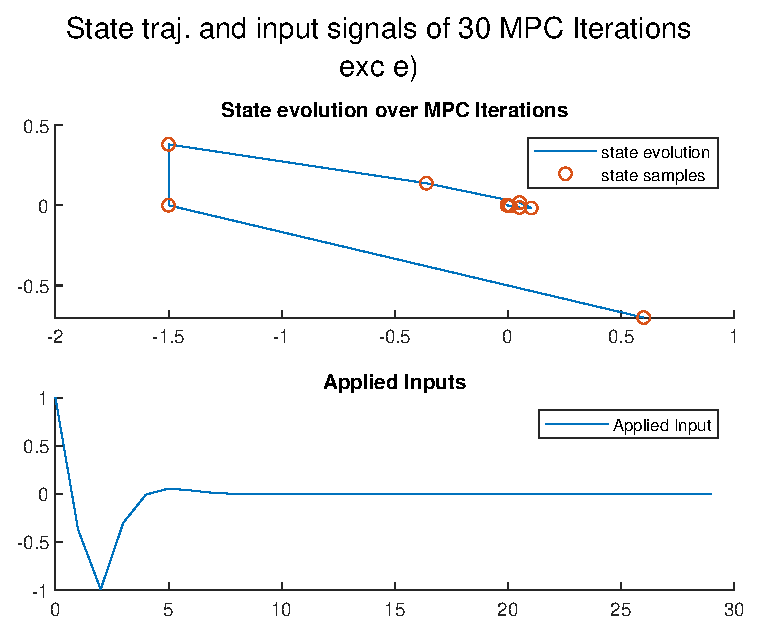
\includegraphics[width=0.9\linewidth]{plots/exc_e}
					\caption[Plot for exc. e)]{Plot for exc. e)}
					\label{fig:exce}
				\end{figure}}
		{	\item[f)]
			\begin{figure}[H]
				\centering
				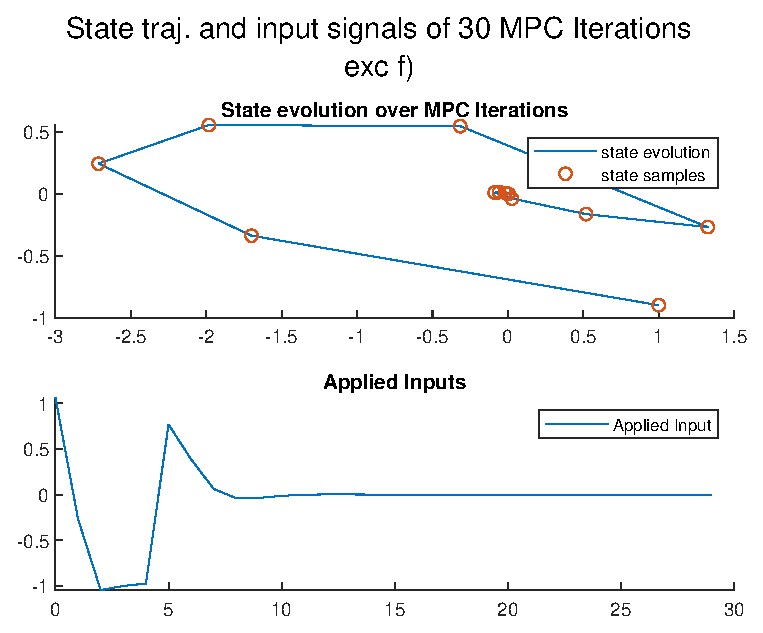
\includegraphics[width=0.9\linewidth]{plots/exc_f}
				\caption[Plot for exc. f)]{Plot for exc. f)}
				\label{fig:excf}
			\end{figure}}
					
		\end{enumerate}	
		
\end{document}
